
\chapter{DEVELOPMENT OF A MULTIPLE-MINIMA FLUCTUATING CHARGE (MM-FLUCQ) POTENTIAL}
\label{chap:mmFlucQ}


In this chapter the initial development of the mm-FlucQ potential will be
presented. Preliminary results of charged species approaching the \ce{Pt}
surface will also be examined. Finally, current challenges and future
directions will be discussed.


\section{Introduction}
Metal surfaces and interfaces play a key role in a number of chemical and
technological processes; however, the tendency of oxide layers to form on these
interfaces requires a more complete picture when describing adhesion and
interactions at the surface. The modified atomistic structure of these surface
after oxide formation is expected to affect many properties of the interface,
especially the local electric field, but also diffusion and adsorption on the
surface.\citep{Bray:2011hq,Small:2012dw,Streitz:1994mw}

Treating the electrodynamics of such a system within molecular dynamics is a
challenging problem. Whereas non-metallic species can be modeled satisfactorily
with static point charges, metals and metal oxides require a more complicated
description of the electrostatic interactions. The idea of electronegativity
equalization introduced by Sanderson\citep{Sanderson:1951mz} provides a
framework that allows charge transfer between both atomic and molecular
species. In this formalism, as a species gains negative charge, its electronegativity
decreases, similarly, if an atomic site has lost charge, then it has an
increased electronegativity. The system would then only be at a charge
equilibrium if all of the electronegativities were equal. It is helpful to
remember that the electronegativity, $\chi_A$, as defined by
Mulliken\citep{Mulliken:1934wt} is equal to the negative of the chemical
potential, $\mu_A$, of the valence electron gas around a positive nucleus
nucleus as shown by Iczkowski and Margrave\citep{Iczkowski:1961wq},
\begin{equation}
\chi_A = -\mu_A = -\frac{\partial E}{\partial N}
\end{equation}
where $E$ is the ground state energy of the atom and $N = n - Z$ where $Z$ is
the atomic number and $n$ is the number of electrons around the nucleus. Thus
$N = 0$ for the neutral species, $+1$ for the positive ion, and $-1$ for the
negative ion.  This description implies that upon movement of the nuclei, the
electrons will instantaneously move so as to equilibrate the electrochemical
potential. Rick {\it et al.} in their work on fluctuating charge water
allowed the atomic charges to fluctuate dynamically by coupling the
electronegativity equalization method with a fictitious charge variable on each
atomic site. This charge variable $Q_A$ was then propagated with the rest of
the dynamics of the system by using an extended Lagrangian
approach.\citep{Rick:1994ss}.

The basic idea of a dynamic fluctuating charge model is to allow partial
charges on atomic sites to become dynamical variables.  Each atomic site
therefore has four ``position'' variables, $\{\vec{\mathbf{r}}_A, Q_A\}$, and
four velocities, $\{\dot{\vec{\mathbf{r}}}_A, \dot{Q}_A\}$.   In addition to
standard electrostatic interactions between the dynamic fluctuating charges,
there is a self energy term that must be taken into account. Similar to Rapp\'e
and Goddard\citep{Rappe:1991dq} we make use of a Taylor expansion around the
neutral species with respect to charge.  This self term through second order
leads to,
\begin{equation} \label{eqn:selfenergy}
E_A(Q_A) = E_{A_0} + Q_A\bigg( \frac{\partial E}{\partial Q} \bigg )_{A_0} +
\frac{1}{2}Q_A^2 \bigg(\frac{\partial^2E}{\partial Q^2}\bigg)_{A_0}
\end{equation}
where $E_{A_0}$ is the ground state energy of the neutral species, $A$, and the higher order terms
are shown to be the electronegativity, $\chi$, and electronic hardness, $J$, as derived below,
\begin{align*}
\mathrm{IP} &= E_A(+1) - E_A(0) \\
& = E_{A_0} + \bigg (\frac{\partial E}{\partial Q}\bigg)_{A_0} + \frac{1}{2}\bigg(\frac{\partial^2E}{\partial Q^2}\bigg)_{A_0} - E_{A_0} \\
\mathrm{EA} &= E_A(0) - E_A(-1) \\
& = E_{A_0} - E_{A_0} + \bigg (\frac{\partial E}{\partial Q}\bigg)_{A_0} - \frac{1}{2}\bigg(\frac{\partial^2E}{\partial Q^2}\bigg)_{A_0}  \\
\bigg (\frac{\partial E}{\partial Q}\bigg)_{A_0} &= \frac{\mathrm{IP+EA}}{2} = \chi_A \qquad \bigg (\frac{\partial^2 E}{\partial Q^2}\bigg)_{A_0} = \mathrm{IP-EA} = J_A
\end{align*}
where IP is the ionization potential and EA is the electron affinity of species $A$.  This
description allows us to rewrite equation \ref{eqn:selfenergy} with the following,
\begin{equation}
E_A(Q_A) = E_{A_0} + \chi_A Q_A + \frac{1}{2} J_{A} Q_A^2
\end{equation}


The electronegativity $\chi$ is well-described by
$\frac{\mathrm{IP+EA}}{2}$; whereas, the electronic hardness term is often approximated using
Rapp\'e and Goddard's approach, where $J$ is equal to the
Coulomb overlap integral between Slater orbitals centered on each
atomic site\citep{Rappe:1991dq}.

The harmonic self energy expression is enormously useful. Even in
large systems of coupled fluctuating charge sites, the charges move on
a purely harmonic ``bowl'' where the minimum energy state for the
system of charges can be determined uniquely. Charge conservation
constraints can be applied to a constrained electronegativity
equalization procedure to find the best set of charges for a given set
of nuclear positions.  Additionally, motion of the atomic sites simply
changes the location of the minimum and curvature of the charge bowl,
but these are relatively smooth variations, allowing standard
integration techniques to be used to propagate the charge variables.

One limitation of the harmonic self-interaction potential is the
inability to represent multiple stable oxidation states of various
species. In many simple molecules or ions, only one dominant oxidation
state is present, but at the surfaces of metals (and particularly
during metal oxide formation), there can be multiple oxidation states
(e.g. \ce{Pt^0}, \ce{Pt^2+}, \ce{Pt^4+}, etc.) present in the system simultaneously.

Another weakness of the harmonic approach is the reliance on the unit
charge gas phase ions in determining the first and second derivative terms, $\chi$ and $J$.  In
many charge partitioning schemes (and in most classical force fields),
the partial charges assigned to condensed phase atoms are
significantly smaller than the unit charges required to produce the gas phase
ions, e.g. the \ce{H} in \ce{H2O} in TIP4P is assigned a charge of +0.52.\citep{}  This
results in electronegativity and hardness terms that may be poor estimates of the local
slope, and harmonic wells that are overly broad.

The method we present here builds on the fluctuating charge
method of Rick {\it et al.}\citep{Rick:1994ss}, but models the self energy more
generally using multiple stable ionic states.  This multiple-minimum
fluctuating charge method (mm-flucq) effectively allows for charge
transfer between ionic and metallic species.

\section{Development of methodoloy}

The Lagrangian describing our system, similar to Rick {\it et al.}\citep{Rick:1994ss} is

\begin{equation}
L = \sum^{N_{molec}}_{i=1}\sum^{N_{atom}}_{\alpha = 1} \frac{1}{2}m_{\alpha} \dot{r}^2_{i\alpha} + \sum^{N_{molec}}_{i=1}\sum^{N_{atom}}_{\alpha = 1} \frac{1}{2}M_Q\dot{Q}^2_{i\alpha} - U[(\mathbf{Q}),(\mathbf{r})] - \lambda \sum^{N_{molec}}_{i=1}\sum^{N_{atom}}_{\alpha = 1} Q_{i\alpha}
\end{equation}

where the mass of an atomic site $\alpha$ is defined as $m_\alpha$ and $M_Q$ is
the fictitious charge mass with units of $\frac{\mathrm{energy\times
time}^2}{\mathrm{charge}^2}$, or more specifically, $\frac{\mathrm{kcal\times
fs}^2}{\mathrm{mol\times e}^2}$


The potential energy term $U[(\mathbf{Q}),(\vec{\mathbf{r}})]$ contains the expected
pieces from standard molecular dynamics simulations, $U_{\text{bonds}},
U_{\text{bends}}, U_{\text{torsions}}, U_{\text{electrostatic}},
U_{\text{Lennard Jones}}$ etc. It also contains the new self energy term necessary
for modeling dynamic fluctuating charges. This term, instead of using the harmonic
approximation, includes multiple diabatic states,

\begin{equation}
U(Q)_{\text{mm-flucq}} =
\begin{Bmatrix}
 V_0(Q) & c  \\
 c   & V_1(Q)
\end{Bmatrix}
\end{equation}

Where $c$ is a coupling constant between states $i$ and $j$, and $V_i(Q)$ is seen below,

\begin{equation*}
V_i(Q) = \frac{1}{2}k(Q - Q_i)^2 + V_i
\end{equation*}

Each diabatic state, $V_i(Q)$ treats the local energy around a stable charge
site, $Q_i$, as a harmonic function that is scaled by $k$ and offset by $V_i$.
However, by constructing our self-potential energy landscape out of many
diabatic states, we are able to create a surface with multiple charge minima.
An ideal multiple-well potential is shown in Figure \ref{fig:multipleDiabat}.
This method can be extended by adding more diabatic states as shown in the
following matrix.

\begin{figure}
  \centering
  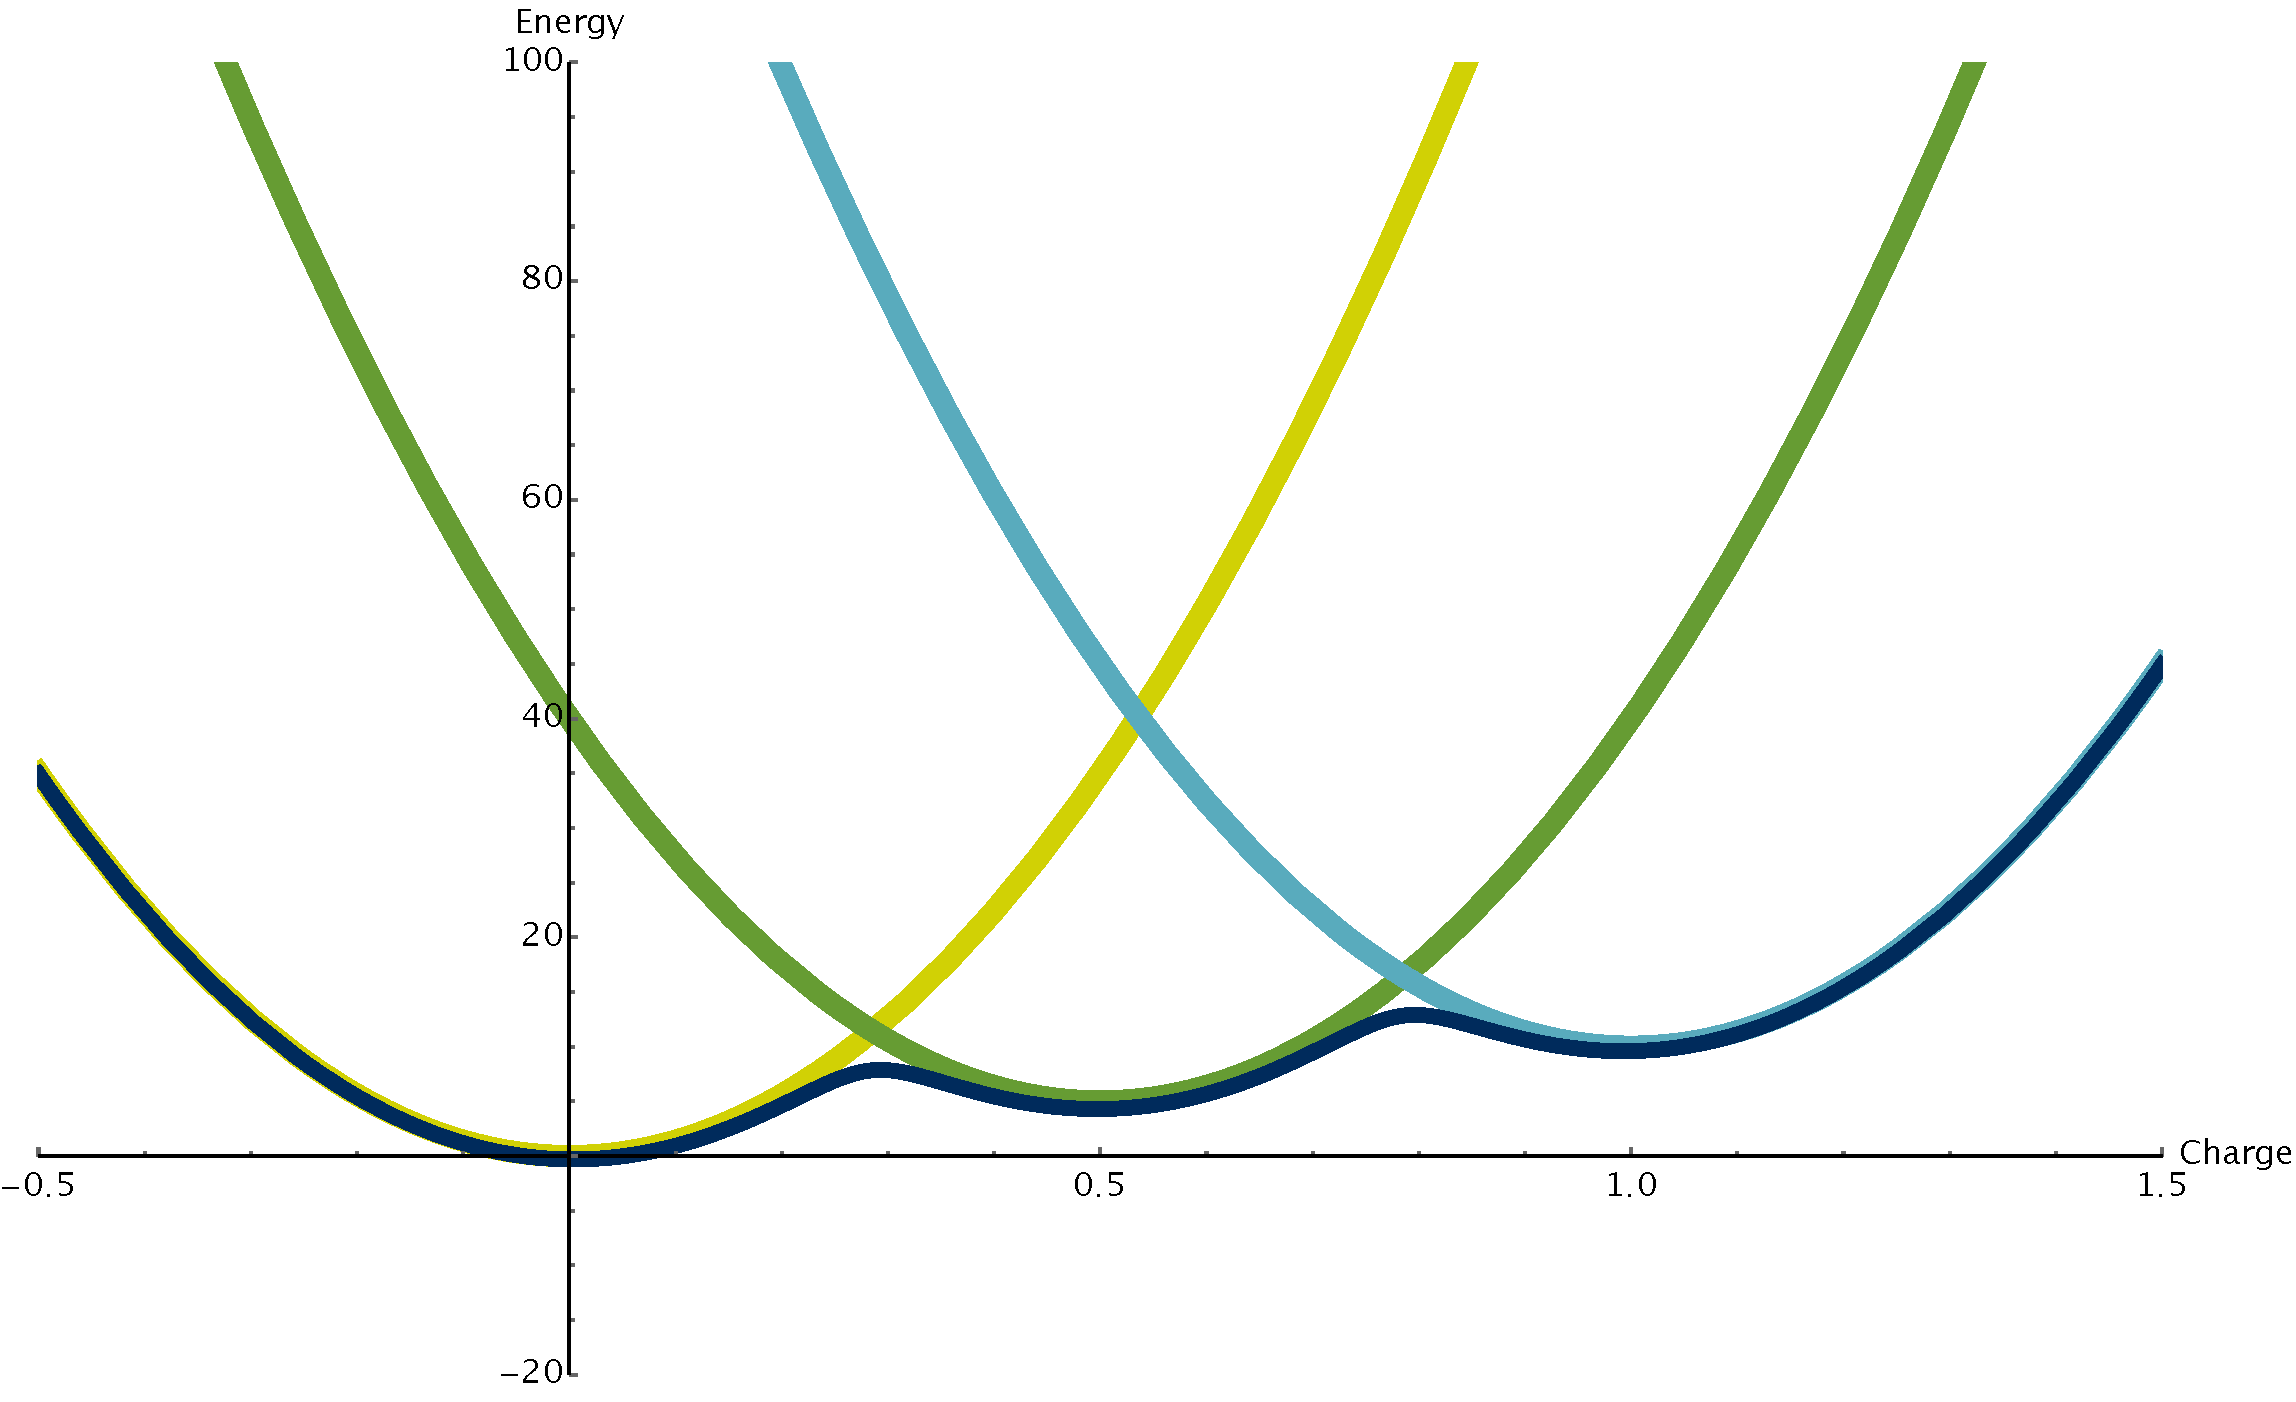
\includegraphics[width=0.75\linewidth]{../figures/chap5/multipleDiabats.pdf}
  \caption{The gold, green, and cyan curves represent the diabatic energies
while the navy triple-well potential was created using the following parameters.
$[Q_0 = 0, Q_1 = 0.5, Q_2 = 1, V_0 = 0, V_1 = 5, V_2 = 10, k = 280, c = 3.5]$}.
\label{fig:multipleDiabat}
\end{figure}

\begin{equation}
  \begin{Bmatrix}
    V_0(Q) & c      & 0      & \dots  & 0\\
    c      & V_1(Q) & c      & \dots & 0\\
    0      & c      & V_2(Q) & \ddots & 0 \\
    \vdots & \vdots & \ddots & \ddots & c\\
    0      & 0      & 0      &  c     & V_n(Q) \\
    \end{Bmatrix}
\end{equation}

\subsection{Parameterization}
One weakness of this proposed method is the need for a large number of
parameters.  Currently, even with assumptions made about the coupling constant
$c$ not differing between states and there being no coupling between states
when $|i-j| > 1$  and $k$ being the same for all of the individual diabatic
states there will still need to be $2n+2$ parameters depending on the number, $n$, of
diabatic states the system requires to properly model its electronic
environment.

\begin{equation*}
\text{Parameters} = [Q_0 \dots Q_n, V_0 \dots V_n, k, c] = \text{2n+2}
\end{equation*}

A more complicated example of a charge surface with best-guess parameters is
that of oxygen in an oxide system.  The ``stable'' charge position of the wells
were obtained from a set of DFT calculations performed on the platinum oxide
surface. Bader charge analysis was performed and a histogram was generated
based on the populations of oxygen and platinum in various charge states. The population analysis
is shown in figure \ref{fig:population}. A first attempt at the interaction
potential was then created and is shown in Figure \ref{fig:Ocharge}.

\begin{figure}
  \centering
  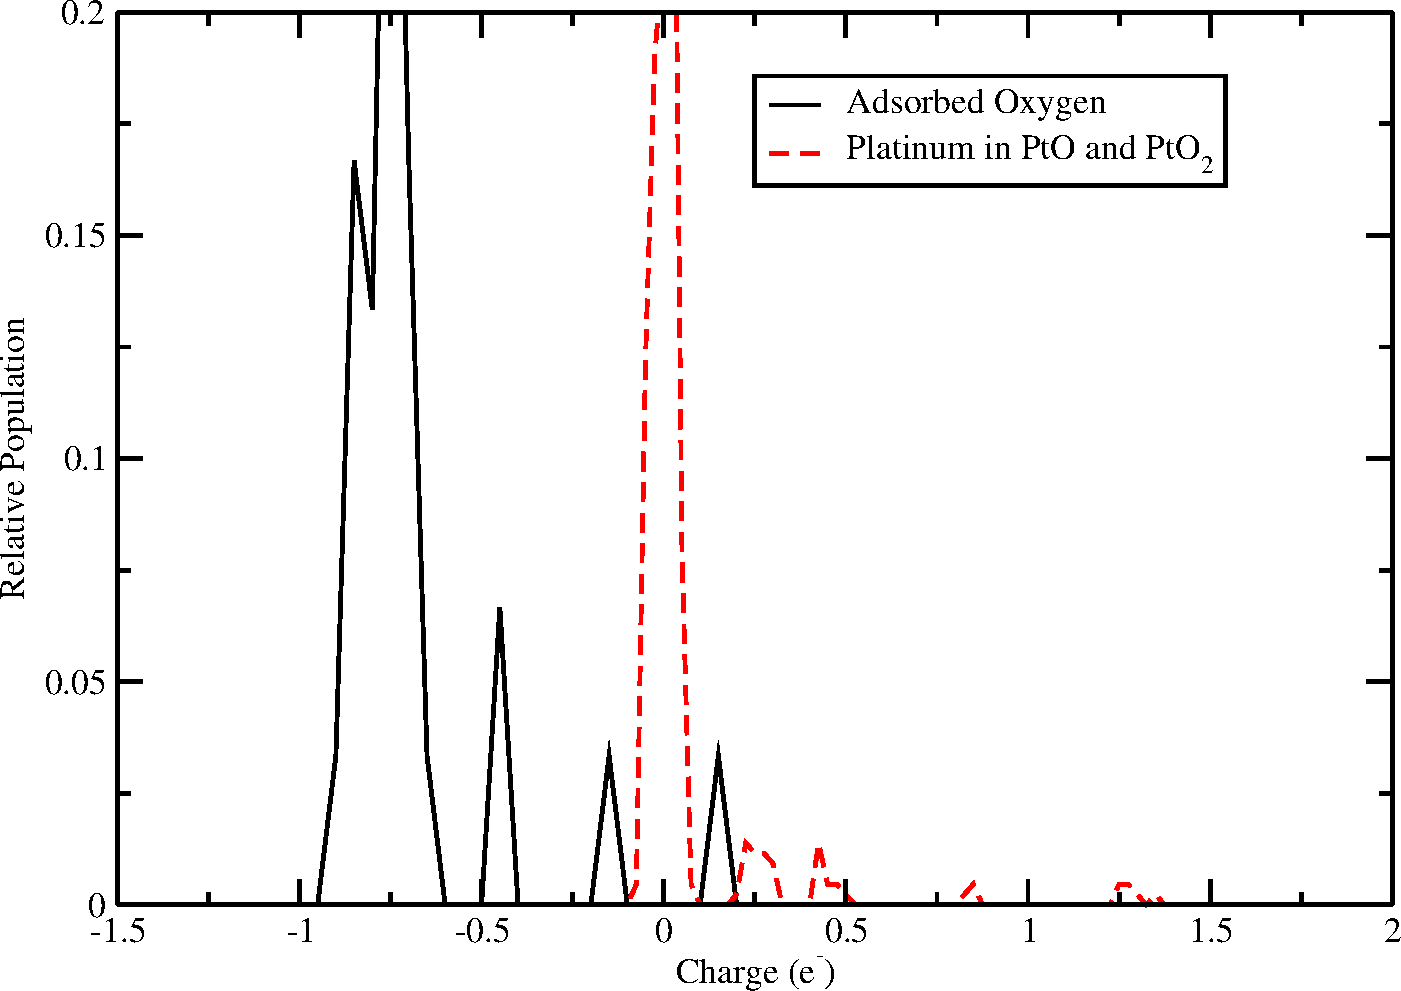
\includegraphics[width=0.75\linewidth]{../figures/chap5/chgDist_PtO.pdf}
  \caption{Histogram of oxygen and platinum charges obtained from a sampling of platinum oxide DFT calculations.}
\label{fig:population}
\end{figure}

\begin{figure}
  \centering
  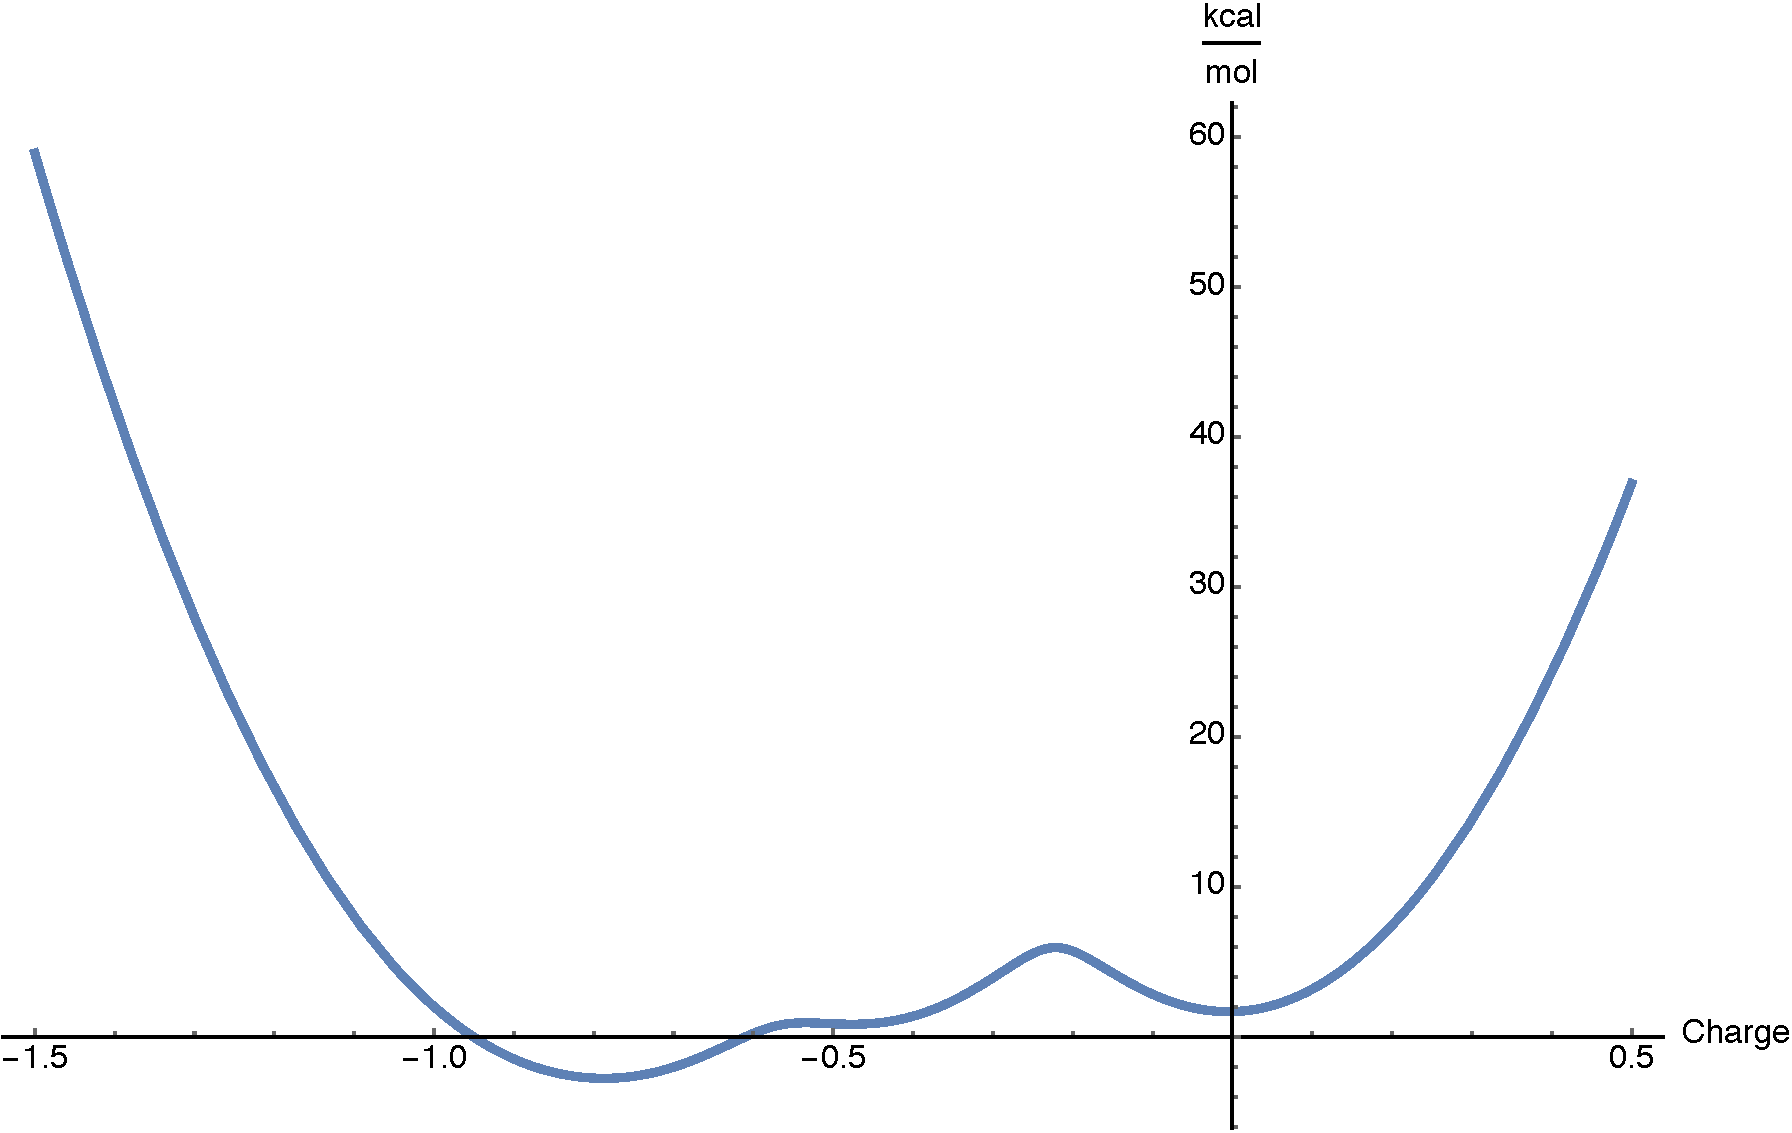
\includegraphics[width=0.75\linewidth]{../figures/chap5/Oxygen_Charge_Testing.pdf}
  \caption{A possible description of the self-interaction oxygen charge
potential. The parameters to generate this potential are $[Q_0 = -0.85, Q_1 =
-0.75, Q_2 = -0.45, Q_3 = 0, V_0 = 0.25, V_1 = 0, V_2 = 2, V_3 = 2, k = 280, c
= 3]$.}
\label{fig:Ocharge}
\end{figure}

A similar attempt was made to create an interaction potential for \ce{Pt} and
is seen in Figure \ref{fig:PtCharge}. The current approach attempts to minimize
the contribution from the vast majority of Platinum that stay near $0$ charge.

\begin{figure}
  \centering
  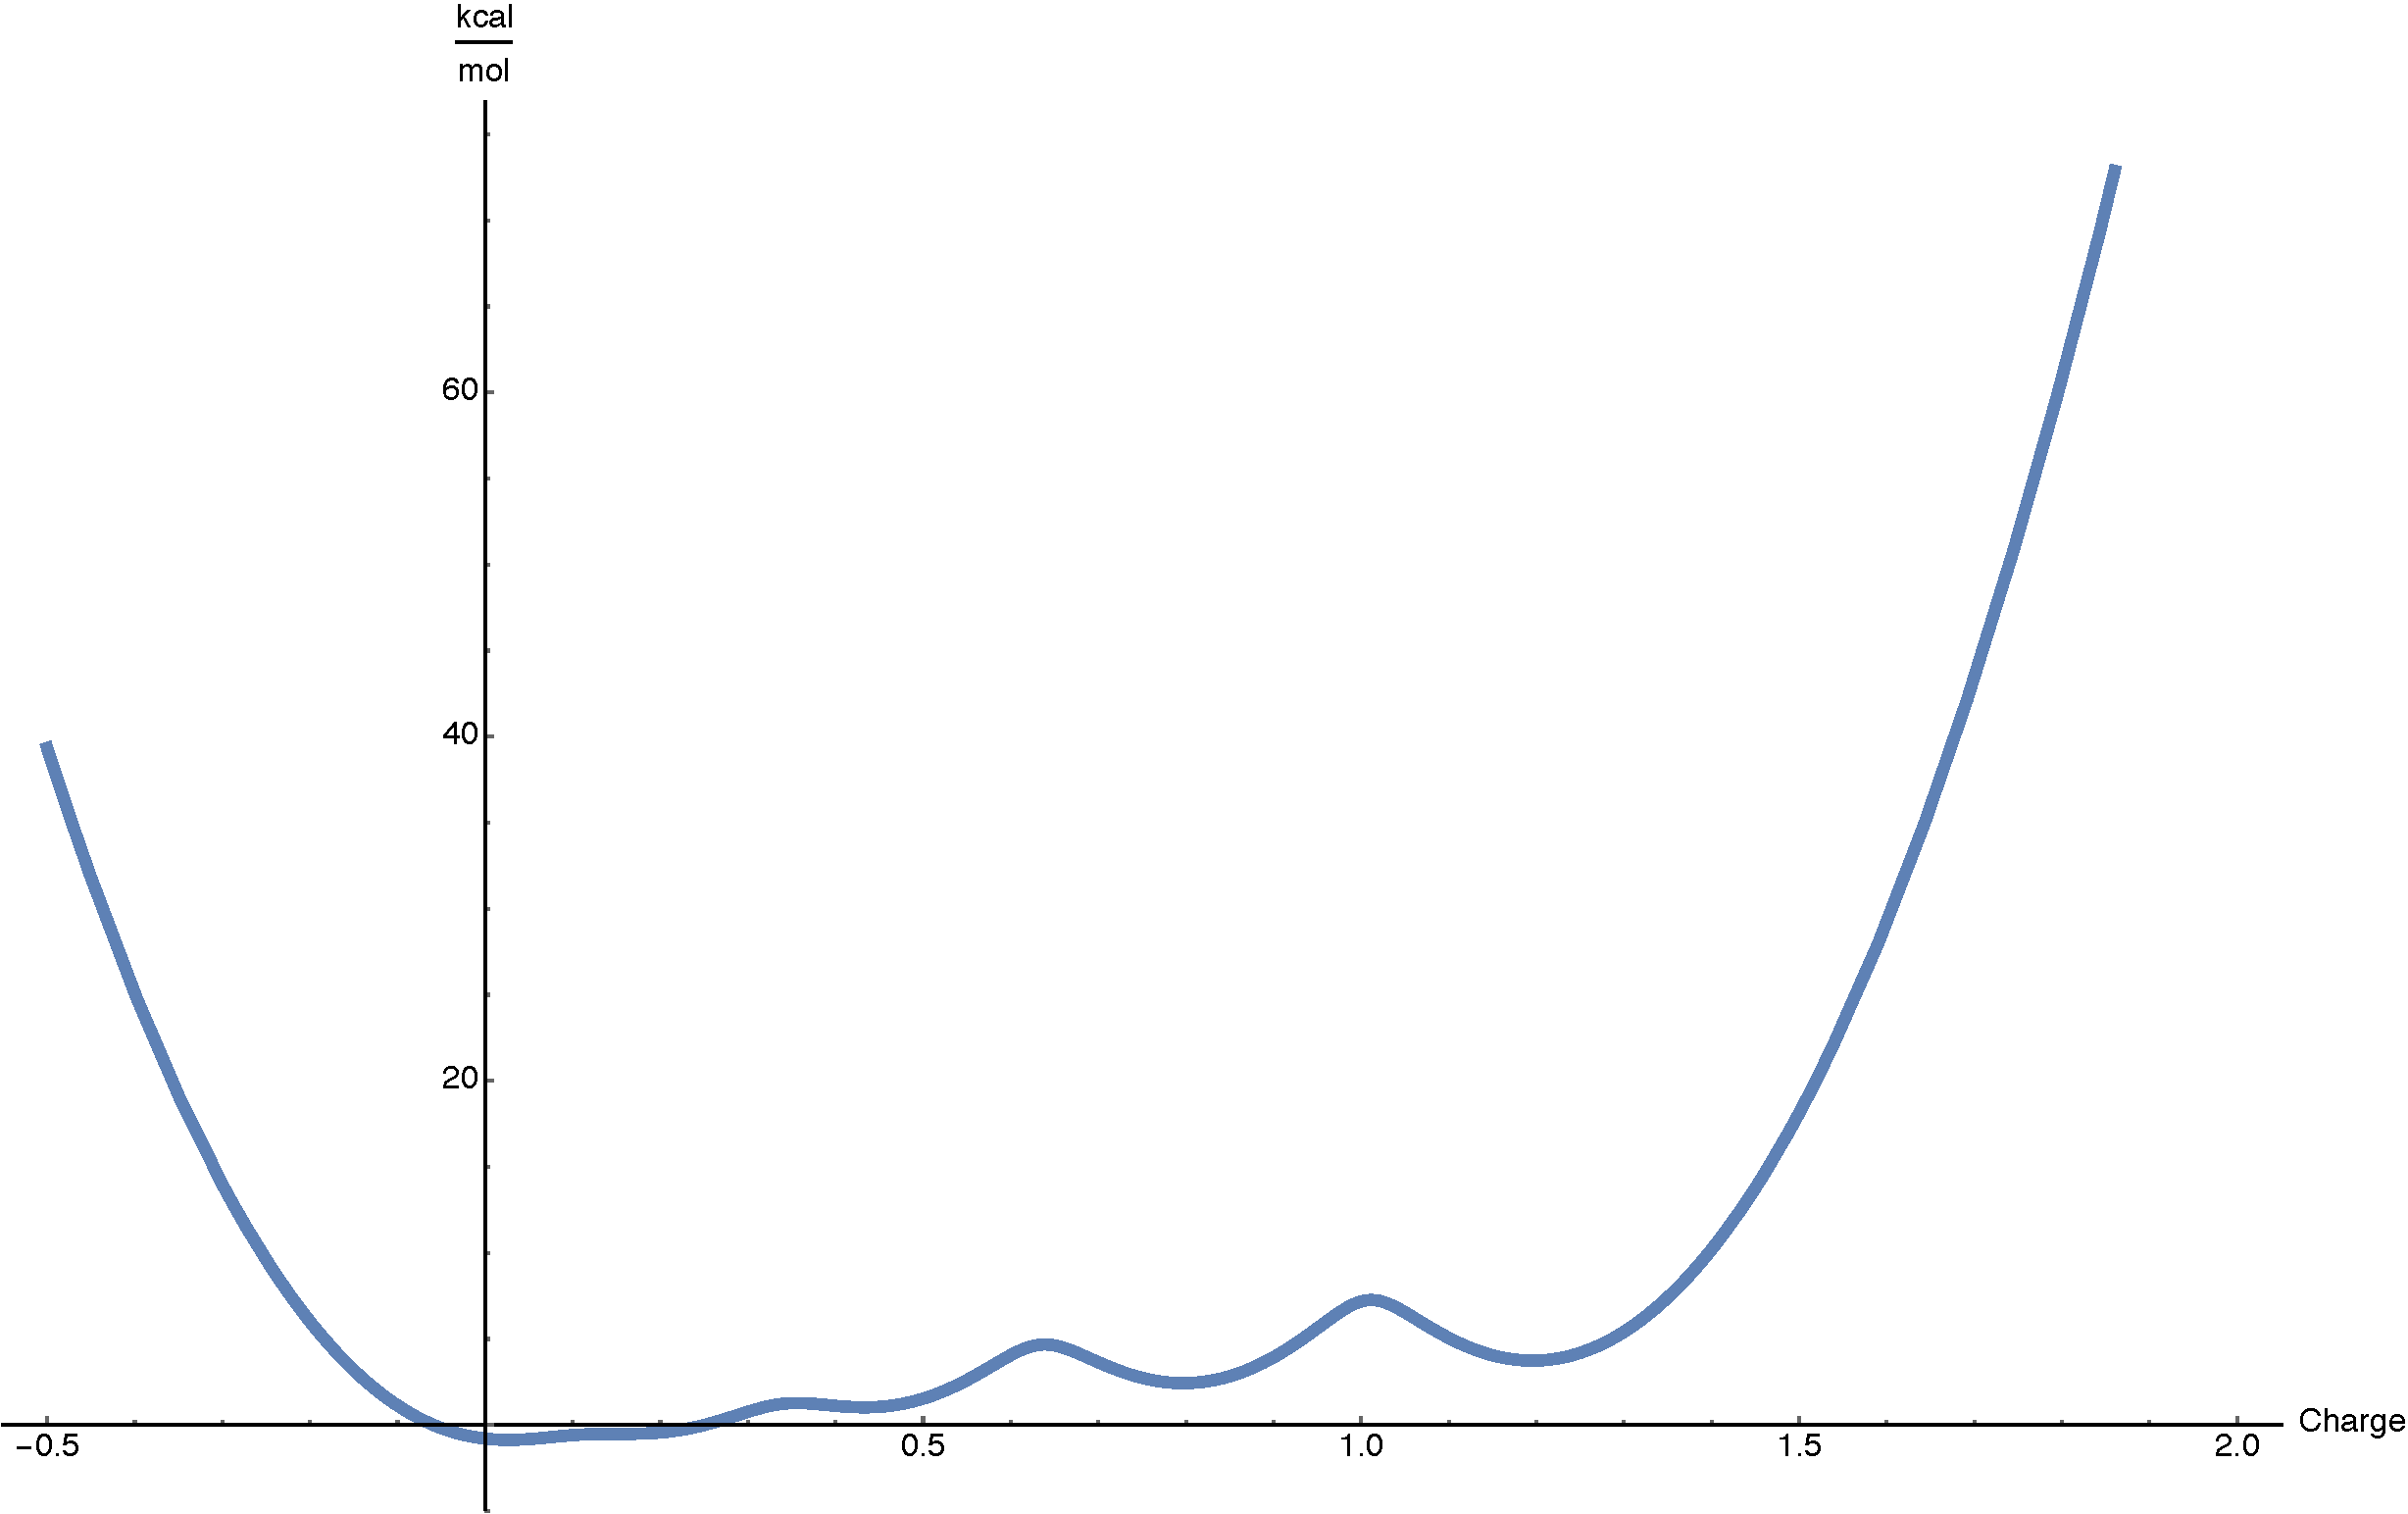
\includegraphics[width=0.75\linewidth]{../figures/chap5/Pt_Charge_Testing.pdf}
  \caption{Parameters: $[q_0 = 0, q_1 = 0.2, q_2 = 0.45, q_3 = 0.8, q_4 = 1.2, V_0 = 0, V_1 = 1, V_2 = 2, V_3 = 3, V_4 = 4, k = 316, c = 2.5]$}
\label{fig:PtCharge}
\end{figure}

Using the population analyses to determine valid charge states allows us to
parameterize the $Q_n$ values. The coupling constant $c$ currently has no
experimental justification and is tuned to ensure that a smooth potential is
obtained to minimize issues with integrating the dynamics. The scaling constant
$k$ has been obtained from the atomic/molecular polarizability by using an
ideal two particle system and is explained more fully in the next section.
Finally, the relative energies $V_n$ are currently being arbitrarilly set until we are able to provide 
theoretical or experimental justifications.


\subsection{Determining $k$}
To determine the value for $k$, the scaling parameter in this scheme, we first
created an ideal two-particle system separated by $a_o$, as illustrated in the cartoon below.
We then arbitrarilly shifted one unit of charge between
the otherwise identical atoms. We then described the Hamiltonian of the system as follows.
\begin{figure}
  \centering
  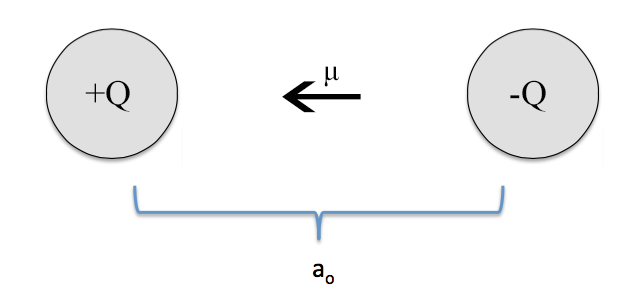
\includegraphics[width=0.75\linewidth]{../figures/chap5/determineK2.png}
\end{figure}

\begin{equation*}
H = f_1(+Q) + f_2(-Q) - \frac{Q*Q}{4\pi\varepsilon_o a_o} - \mu\cdot\vec{E}
\end{equation*}

Where $f_1(Q)$ describes the kinetic and simplified self-potential of the
atom's charge and is shown below,

\begin{equation*}
f(Q) = \frac{P_Q^2}{2m_Q} + \frac{1}{2}kQ^2
\end{equation*}

where $P_Q$ represents the ``momentum'' and $m_Q$ the mass of the charge while
$k$ is the scaling factor we are deriving. The electrostatic interaction term
and the dipole moment of the system interacting with the local electric field
complete our description of our model. Rewriting the kinetic terms as $T$,
combining like terms, and replacing $\mu$ with $Q\cdot a_o$ leads to the
following.

\begin{equation*}
H = T + Q^2\bigg(k - \frac{1}{4 \pi\varepsilon_o a_o}\bigg) - Q\cdot a_o \cdot \vec{E}
\end{equation*}

The right two terms are a shifted harmonic oscillator and can be solved in the
following manner after replacing $k-\frac{1}{4\pi\varepsilon_o a_o}$ with $a$
and $a_o\cdot \vec{E}$ with $b$.

\begin{equation*}
T + aQ^2 - bQ  = T + a\bigg(Q^2 - \frac{b}{a}Q\bigg) = T + a\bigg(\bigg(Q^2 - \frac{b}{a}Q + \frac{b^2}{4a^2}\bigg) - \frac{b^2}{4a^2}\bigg)
\end{equation*}

Taking the derivative of $H$ with respect to $Q$ to find the minimum results in $Q = \frac{b}{2a}$,
which when replacing $a$ and $b$ with their original values provides us with
the following equation for $Q_{\text{min}}$.

\begin{equation*}
Q_{\text{min}} = \frac{a_o \cdot \vec{E}}{2(k - \frac{1}{4\pi\varepsilon_o a_o})}
\end{equation*}

Recalling that the effective dipole moment is equal to $\mu_{\text{eff}} =
Q_{\text{min}}\cdot a_o$ and $\mu = \alpha\vec{E}$ where $\alpha$ is the atomic
polarizability, we reach the following solution in terms of $k$.

\begin{equation*}
k = \frac{a_o^2}{2\alpha} + \frac{1}{4\pi\varepsilon_o a_o}
\end{equation*}

Using a polarizability for Pt of $\alpha = 6.5$ \AA\textsuperscript{3} and a
nearest neighbor distance of $2.77$ \AA~we obtained a value for $k$ of 316
$\frac{\text{kcal}}{\mathrm{mol\times e}^2}$. Various polarizabilities and
distances can be obtained for oxygen binding to platinum but all of the results
end up around 280 $\frac{\text{kcal}}{\mathrm{mol\times e}^2}$ for a value of
$k$. These values are meant to be used as starting points for the
parameterization rather than as fixed points since the system used to derive
these values is an idealized model and not descriptive of the systems we
examined.

\section{Preliminary Results}

The mm-flucq method continues to assume that a species electrons are collapsed
as point charges on the atomic sites. We currently do not allow for anisotropy and assume
that the electron density decays in a radial fashion. To visualize the charge density in these systems we treat the
density at a site $i$ with a three dimensional gaussian function as shown
below,
\begin{equation*}
\rho(\vec{\mathbf{r}}) = \sum_i q_{i} \frac{1}{(2\pi)^{3/2}}e^{\frac{-(\vec{\mathbf{r}}-\vec{\mathbf{r}}_i)^2}{2}}
\end{equation*}
where our isotropic requirement leads to $\sigma_x = \sigma_y = \sigma_z = 1$,
$q_i$ is the charge of atom $i$ and $\Delta r$ is the distance from the point
where the density is being measured to the position of the atomic site
$\vec{\mathbf{r}}_i$.

Our visualization method begins with defining a uniform grid of points (spacing
approximately 1 \AA) spread throughout the simulation box. The electron density
as contributed by nearby atomic sites is summed at each grid point and then
assembled to use in a volume rendering program, e.g. Amira. As seen in figure
\ref{fig:chargeVol}, which depicts a \ce{Cl-} ion approaching a charge responsive
\ce{Pt} surface, most of the metal atoms experience minimal disruption away
from the neutral ground state, whereas the metal directly beneath the \ce{Cl-}
ion gains a significant amount of positive charge. The units of the charge
density are $e^{-}$/\AA\textsuperscript{3} as calculated from the above gaussian.
Figure \ref{fig:chargeHistogram} provides another view of this system by
looking at the charge population of the \ce{Pt} at various times over the
simulation length.

\begin{figure}
  \centering
  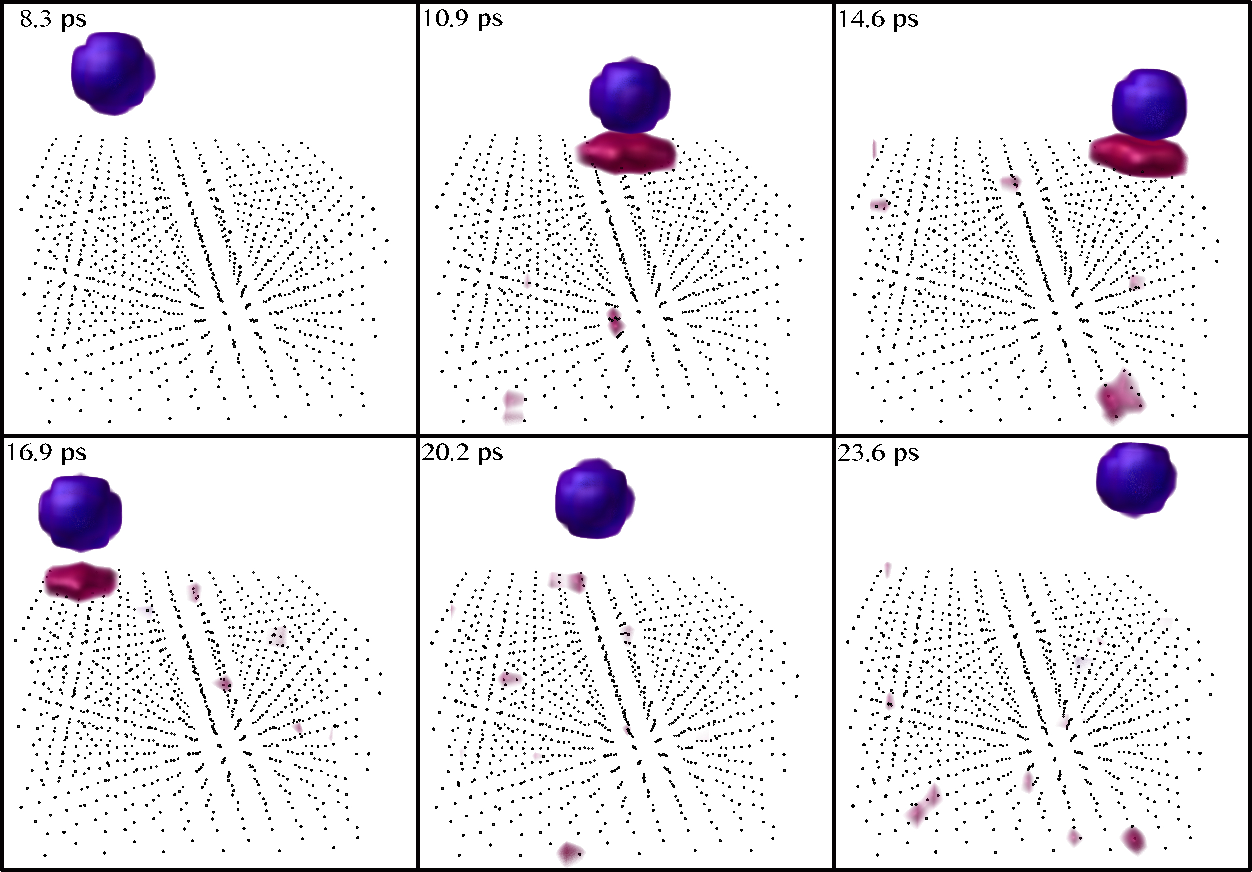
\includegraphics[width=0.75\linewidth]{../figures/chap5/PtOChargeVolume.pdf}
  \caption{As the \ce{Cl-} approaches the surface, the \ce{Pt} directly beneath
the \ce{Cl-} loses electron density leading to a favorable interaction between
the \ce{Pt} and \ce{Cl-}. To maintain charge neutrality, the surrounding
\ce{Pt} receives a slightly negative charge as illustrated by the less defined
purple cloud around the positive charge site. Units are in
$e^-$/\AA\textsuperscript{3}.}
\label{fig:chargeVol}
\end{figure}

\begin{figure}
  \centering
  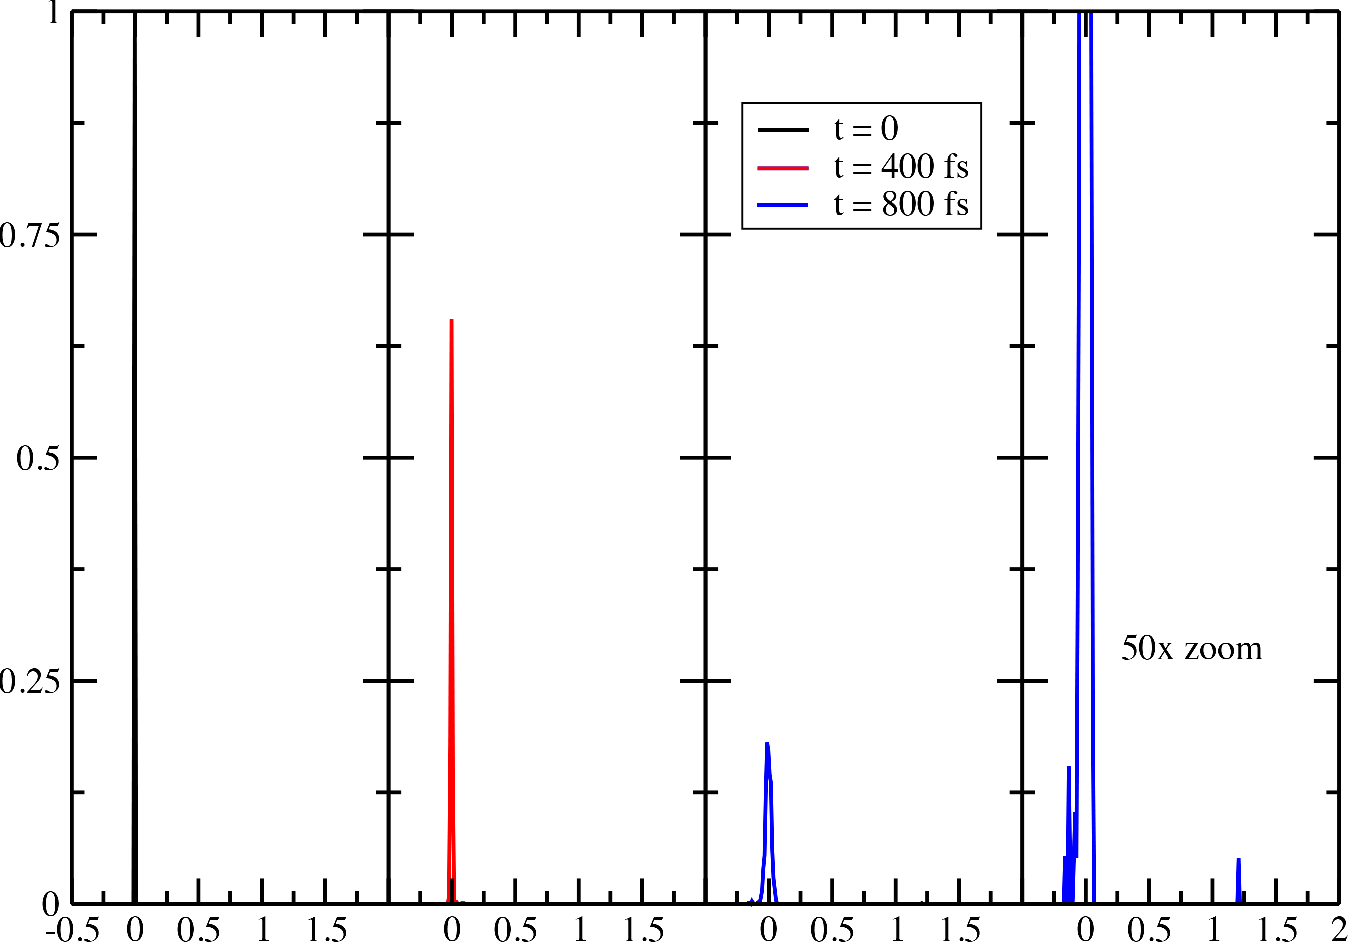
\includegraphics[width=0.75\linewidth]{../figures/chap5/chargeHistogram.pdf}
  \caption{As \ce{Cl-} approaches the surface the initially neutral \ce{Pt}
begins to experience small fluctuations about 0 charge. The fourth panel shows
the data at 800 fs magnified by a factor of 50 and shows a small peak at
approximately +1.2 charge which corresponds to the accumulation of positive
charge directly beneath the \ce{Cl-}. There is also a slight shifting of the
remaining \ce{Pt} towards small negative charges so as to maintain charge
neutrality in the system.}
\label{fig:chargeHistogram}
\end{figure}


\section{Future Directions}
While this method has succeeded in capturing the movement and accumulation of
charge in a metal surface in response to an incoming ion, accurate
parameterization of the numerous parameters in equation \ref{eq:} is still
on-going. Additionally, the build-up of charge directly at the surface, rather
than at a distance $d$, where $d$ is the distance of the charged adsorbate away
from the surface, as predicted by the method of images suggests that further
work is needed to properly incorporate the electric potential being constant at
the surface. This work is on-going and when completed opens up a large realm of
possible directions of studies.

Adsorbate interactions with metal surfaces is one of the first class of
problems that will be explored with this technique and will include small
molecules, {\em i.e.} \ce{CO}, \ce{H2O}, \ce{NO}, etc., metal ions, and small
biological analogs. Capturing the formation of oxides is also one of the future
goals for this project. 



